\documentclass[10pt,a4paper]{article}
% ---------- common preamble : CM3191 organic documents (XeLaTeX) ----------
\usepackage[a4paper,top=16mm,bottom=16mm,left=16mm,right=16mm,headheight=14pt]{geometry}
\usepackage{fontspec}
\usepackage{xeCJK}
\setmainfont{TeX Gyre Termes}
\setsansfont{TeX Gyre Heros}
\setCJKmainfont{Noto Serif CJK KR}
\setCJKsansfont{Noto Sans CJK KR}
\xeCJKsetup{CJKspace=true, CJKecglue={}}
\usepackage{amsmath,amssymb}
\usepackage[version=4]{mhchem}
\usepackage{chemfig}
\usepackage{siunitx}
\sisetup{detect-all, per-mode=symbol, range-phrase=--, range-units=single}
\usepackage{tikz}
\usetikzlibrary{arrows.meta,calc,positioning,shapes.geometric,decorations.pathmorphing,patterns}
\usepackage{tabularx,array,multirow,booktabs}
\usepackage{enumitem}
\usepackage{titlesec}
\usepackage{fancyhdr}
\usepackage{xcolor}
\usepackage{pifont}
\usepackage[hidelinks]{hyperref}
\setlength{\parindent}{0pt}
\setlength{\parskip}{3pt}
\linespread{1.08}

\newcommand{\doctag}{}
\pagestyle{fancy}\fancyhf{}
\lhead{\footnotesize CM3191 Organic \textemdash\ \doctag}
\rhead{\footnotesize KIM DONGHWAN \textbullet\ B7 \textbullet\ Thu}
\cfoot{\footnotesize \thepage}
\renewcommand{\headrulewidth}{0.4pt}

\titleformat{\section}{\large\bfseries}{\thesection}{0.6em}{}
\titlespacing*{\section}{0pt}{9pt}{4pt}
\titleformat{\subsection}{\normalsize\bfseries}{\thesubsection}{0.5em}{}
\titlespacing*{\subsection}{0pt}{7pt}{3pt}

% ---------- form primitives ----------
\newcommand{\wl}[1][4cm]{\rule[-0.6ex]{#1}{0.4pt}}
\newcommand{\cbox}{$\square$}
\newcommand{\tr}{\rule[-3mm]{0pt}{9mm}}
\newcommand{\trs}{\rule[-2mm]{0pt}{7mm}}
\newcommand{\ruled}[1]{%
  \par\vspace{3mm}%
  \foreach \i in {1,...,#1}{\noindent\rule{\linewidth}{0.35pt}\par\vspace{7mm}}%
  \vspace{-7mm}}
\newcommand{\confirm}[1]{\textbf{[CONFIRM: #1]}}

% ---------- boxed callout ----------
\newenvironment{callout}[1]
  {\par\vspace{2mm}\noindent\begin{tabular}{|@{\hspace{2.5mm}}p{\dimexpr\linewidth-7.4mm\relax}@{\hspace{2.5mm}}|}\hline
   \rule{0pt}{4.5mm}\textbf{#1}\par\vspace{0.5mm}\small}
  {\par\vspace{1.5mm}\\\hline\end{tabular}\par\vspace{2mm}}

% ---------- title block ----------
\newcommand{\manualtitle}[3]{%
\begin{center}
{\Large\bfseries #1}\\[1.5mm]
{\large #2}\\[2mm]
{\footnotesize #3}
\end{center}
\vspace{-1mm}\rule{\linewidth}{1pt}\vspace{1mm}
}

% ---------- GTA sign-off ----------
\newcommand{\gtasign}{%
\par\vspace{3mm}
\renewcommand{\arraystretch}{1.4}
\noindent\begin{tabularx}{\linewidth}{|X|X|X|}
\hline
\multicolumn{3}{|l|}{\textbf{To be completed at the end of the session}}\\ \hline
Student signature & GTA name & GTA signature \\ \hline
\tr & & \\ \hline
\end{tabularx}
\renewcommand{\arraystretch}{1}
\par\vspace{1mm}
{\footnotesize This is a working log. The \textbf{official} datasheet (lab manual p.\,7) must still be printed, signed by the GTA and submitted with the report.}
}

% ---------- chemfig defaults ----------
\setchemfig{atom sep=1.9em, bond style={line width=0.6pt}}

\renewcommand{\doctag}{Expt.\ 1 \textemdash\ Suzuki--Miyaura in Water}

\begin{document}

% =====================================================================
% PAGE 1 : PRE-LAB CHECKLIST
% =====================================================================
\manualtitle{ORGANIC EXPERIMENT 1 \textemdash\ PRE-LAB CHECKLIST}
{Suzuki--Miyaura Cross-Coupling in Water: 4-Phenylbenzoic Acid}
{Condensed from the CM3191 Organic Lab Manual AY26/27 (Dr Hoang T.\,G., pp.\,2--7) and lecture CM3191 Org L1. Week 7, \textbf{Thursday 1 October 2026}, Thursday lab (Dr Hoang T.\,G.). Venue \confirm{not stated in the organic schedule}.}

\begin{center}
\setchemfig{atom sep=1.6em}
\schemestart
\chemfig{HOOC-*6(-=-(-Br)=-=)}
\+
\chemfig{*6(-=-(-B(-[:30]OH)(-[:-30]OH))=-=)}
\arrow{->[\footnotesize catalyst \textbf{1} (0.015 mol\%)][\footnotesize \ce{Na2CO3}, \ce{H2O}, 70\,\si{\celsius}, 30 min]}[,2.2]
\chemfig{HOOC-*6(-=-(-*6(-=-=-=))=-=)}
\schemestop
\end{center}

\subsection*{1. Reagent table \ (manual values; blanks in the manual filled by calculation)}
\renewcommand{\arraystretch}{1.25}
\begin{tabularx}{\linewidth}{|X|c|c|c|c|c|}
\hline
\textbf{Reagent} & \textbf{MW / conc.} & \textbf{Amount} & \textbf{mmol} & \textbf{Equiv.} & \textbf{Role} \\ \hline
4-Bromobenzoic acid & 201.02 & 0.34 g & 1.69 & 1.00 & aryl halide (limiting) \\ \hline
Phenylboronic acid & 121.93 & 0.25 g & 2.05 & 1.21 & organoboron partner \\ \hline
\ce{Na2CO3} solution & 0.5 M & 10 mL & 5.0 & 2.96 & base \\ \hline
Pd catalyst solution \textbf{1} & 0.25 mM (Pd) & 1.0 mL & 0.00025 & 0.000148 & catalyst (0.0148 mol\%) \\ \hline
\textbf{4-Phenylbenzoic acid} & 198.22 & \textbf{0.335 g (theor.)} & 1.69 & --- & product \\ \hline
\end{tabularx}
\renewcommand{\arraystretch}{1}

{\footnotesize Theoretical yield = $n(\text{ArBr})\times 198.22$. Recalculate with your \emph{actual} mass of 4-bromobenzoic acid: \quad $m_\text{theor} = m_\text{ArBr}\times(198.22/201.02) = 0.9861\,m_\text{ArBr}$.}

\subsection*{2. Bring / prepare before the session}
\begin{tabularx}{\linewidth}{@{}X X@{}}
\cbox\ Official datasheet (manual p.\,7), \textbf{printed} &
\cbox\ This bench sheet (pp.\,2--5) \\
\cbox\ Lab coat, safety goggles, nitrile gloves, covered shoes &
\cbox\ Phone for photos of every balance reading \\
\cbox\ Labelled plastic bag for product (name) &
\cbox\ Pencil + marker for NMR tube label \\
\cbox\ Know which hotplate is \textbf{shared (70\,\si{\celsius})} vs.\ your own &
\cbox\ NMR solvent: DMSO-$d_6$ \confirm{manual text only says ``the NMR solvent''} \\
\end{tabularx}

\subsection*{3. Session timeline (estimate)}
\renewcommand{\arraystretch}{1.2}
\begin{tabularx}{\linewidth}{|c|X|c|}
\hline
\textbf{\#} & \textbf{Stage} & \textbf{Approx.\ time} \\ \hline
1 & Weigh solids, dissolve in \ce{Na2CO3} (own hotplate, vigorous stirring) & 15 min \\ \hline
2 & Add Pd solution, react in shared 70\,\si{\celsius} block & \textbf{30 min} (fixed) \\ \hline
3 & Cool, acidify with 1 M HCl in ice bath, stir 10 min, suction filter & 25 min \\ \hline
4 & Recrystallize from EtOH (heat, cool to RT 10--15 min, ice 15 min) & 40 min \\ \hline
5 & Suction filter, dry under IR lamp 15 min & 20 min \\ \hline
6 & Weigh, IR, NMR sample, datasheet photo check and GTA signature & 20 min \\ \hline
\end{tabularx}
\renewcommand{\arraystretch}{1}

\begin{callout}{SAFETY \textemdash\ from the manual (p.\,3)}
4-Bromobenzoic acid, phenylboronic acid, \ce{Na2CO3}, the ligand and \ce{Pd(OAc)2} may be harmful if inhaled, swallowed or absorbed through the skin; \ce{Pd(OAc)2} and \ce{Na2CO3} are irritants; the catalyst solution should be considered harmful. NaOH is caustic; HCl is corrosive. Ethanol is highly flammable and a skin/eye irritant. DMSO-$d_6$ is absorbed through the skin and can carry dissolved substances with it. The product is not considered harmful, but avoid inhalation and skin contact. Perform all operations in a well-ventilated fume cupboard.

\textbf{Added notes (not in the manual).} Ethanol is heated to gentle boiling in the recrystallization: hotplate only, no open flames, never heat a closed vessel. Acidification releases \ce{CO2} (the manual's ``gas will form''): add HCl dropwise, in the open conical flask. Waste: Pd-containing aqueous filtrate \textrightarrow\ metal aqueous waste; ethanol mother liquor \textrightarrow\ non-halogenated organic waste. \confirm{waste bins in the organic lab}
\end{callout}

% =====================================================================
% PAGE 2 : ENGLISH BENCH MANUAL
% =====================================================================
\newpage
\manualtitle{BENCH MANUAL (ENGLISH)}{Suzuki--Miyaura Cross-Coupling in Water}{Tick each box as you complete the step. ``Why'' notes explain the purpose; they are not extra steps.}

\subsection*{3.1 Reaction setup}
\begin{enumerate}[leftmargin=7mm,itemsep=1.2mm,label=\cbox\ \arabic*.]
\item Switch on the \textbf{shared} hotplate stirrer with heating block, set \textbf{70\,\si{\celsius}}. \emph{It needs time to equilibrate --- do this first.}
\item Weigh \textbf{0.34 g 4-bromobenzoic acid} and \textbf{0.25 g phenylboronic acid} into a \textbf{20 mL reaction vial}; add a stir bar. Photograph both readings.
\item Add \textbf{10 mL 0.5 M \ce{Na2CO3}}, cap, stir \textbf{vigorously on the hotplate stirrer in your own fume cupboard} (not the shared 70\,\si{\celsius} block) until \textbf{all solids dissolve}.\\
{\footnotesize \emph{Why:} the base converts the acid into its water-soluble sodium carboxylate and activates the boronic acid. The catalyst must not be added until the solution is homogeneous.}
\item Add \textbf{1.0 mL Pd catalyst solution (0.25 mM)}, cap, place in the preheated \textbf{70\,\si{\celsius}} block. \textbf{Start the timer: 30 min.} Record the time.
\end{enumerate}

\subsection*{3.2 Work-up}
\begin{enumerate}[leftmargin=7mm,itemsep=1.2mm,label=\cbox\ \arabic*.,resume]
\item Remove the vial, cool to room temperature, transfer to a \textbf{250 mL conical flask}; stir in an \textbf{ice bath}.
\item Add \textbf{20 mL 1 M HCl slowly, dropwise}, with stirring. \textbf{Gas (\ce{CO2}) forms}; a solid is expected to precipitate.\\
{\footnotesize \emph{Why:} HCl first destroys the carbonate, then protonates the carboxylate; the neutral acid is insoluble in cold water. 20 mmol HCl exceeds the 10 mmol needed for 5 mmol carbonate, so the mixture ends strongly acidic.}
\item Check \textbf{pH paper: acidic}. Add \textbf{20 mL water}; stir \textbf{10 min} in the ice bath.
\item Collect the crude solid by \textbf{suction filtration} (Appendix A).
\end{enumerate}

\subsection*{3.3 Recrystallization (single solvent: ethanol)}
\begin{enumerate}[leftmargin=7mm,itemsep=1.2mm,label=\cbox\ \arabic*.,resume]
\item Crude solid + stir bar into a \textbf{50 mL conical flask} (or a 50 mL beaker). Add \textbf{3 mL 1 M HCl} and \textbf{10 mL ethanol} \ (= solution 1).
\item Second 50 mL conical flask: \textbf{20 mL ethanol} + a few boiling chips \ (= solution 2).
\item Heat both to \textbf{gentle boiling}. With a dropper, add hot ethanol from solution 2 to solution 1 \textbf{only until all solid dissolves} --- use the \textbf{minimum}.\\
{\footnotesize \emph{Why:} every extra mL keeps product in the mother liquor and lowers the yield. The HCl keeps the product fully protonated (neutral acid, not its salt).}
\item Cool \textbf{undisturbed to RT (10--15 min)}, then place \textbf{both} flasks in ice for \textbf{15 min}. \emph{Solution 2 becomes your cold wash solvent.}
\item Suction filter; if necessary, transfer and wash with a \textbf{minimum of cold ethanol} (solution 2).
\item Crystals onto a large filter paper labelled with your name; dry under the \textbf{IR lamp, 15 min}.
\end{enumerate}

\subsection*{3.4 Characterization}
\begin{enumerate}[leftmargin=7mm,itemsep=1.2mm,label=\cbox\ \arabic*.,resume]
\item Weigh the product in a \textbf{pre-weighed plastic bag}; photograph; calculate \% yield.
\item Record an \textbf{IR spectrum}; note the file name.
\item NMR: \textbf{$\sim$10 mg} in a clean, dry plastic vial, dissolve in \textbf{0.6 mL NMR solvent}, transfer with a clean, dry glass dropper; solution height \textbf{$\sim$5 cm} (top up with the same solvent). Cap and label.
\item Show photos to the GTA; get the \textbf{printed official datasheet signed}.
\end{enumerate}

% =====================================================================
% PAGE 3 : KOREAN BENCH MANUAL
% =====================================================================
\newpage
\manualtitle{실험 매뉴얼 (한국어)}{물에서의 Suzuki--Miyaura 교차 커플링}{단계를 마칠 때마다 체크하세요. ``이유''는 목적 설명이며 추가 단계가 아닙니다.}

\subsection*{3.1 반응 준비}
\begin{enumerate}[leftmargin=7mm,itemsep=1.2mm,label=\cbox\ \arabic*.]
\item \textbf{공용} 핫플레이트(히팅 블록)를 켜고 \textbf{70\,\si{\celsius}}로 설정합니다. \emph{온도가 안정되는 데 시간이 걸리므로 가장 먼저 합니다.}
\item \textbf{20 mL 반응 바이알}에 \textbf{4-bromobenzoic acid 0.34 g}, \textbf{phenylboronic acid 0.25 g}, 교반 막대를 넣습니다. 저울 값은 각각 사진으로 남깁니다.
\item \textbf{0.5 M \ce{Na2CO3} 10 mL}를 넣고 뚜껑을 닫은 뒤, \textbf{본인 후드의 교반기}(공용 70\,\si{\celsius} 블록 아님)에서 \textbf{고체가 모두 녹을 때까지} 세게 교반합니다.\\
{\footnotesize \emph{이유:} 염기가 산을 수용성 나트륨 카복실산염으로 바꾸고 보론산을 활성화합니다. 균일한 용액이 되기 전에는 촉매를 넣지 않습니다.}
\item \textbf{Pd 촉매 용액(0.25 mM) 1.0 mL}를 넣고 뚜껑을 닫아 예열된 \textbf{70\,\si{\celsius}} 블록에 올립니다. \textbf{30분 타이머 시작}, 시각을 기록합니다.
\end{enumerate}

\subsection*{3.2 후처리}
\begin{enumerate}[leftmargin=7mm,itemsep=1.2mm,label=\cbox\ \arabic*.,resume]
\item 바이알을 내려 실온으로 식힌 뒤 \textbf{250 mL 삼각플라스크}로 옮기고 \textbf{얼음 수조}에서 교반합니다.
\item \textbf{1 M HCl 20 mL를 한 방울씩 천천히} 넣습니다. \textbf{기체(\ce{CO2})가 발생}하고, 고체가 석출될 것으로 예상됩니다.\\
{\footnotesize \emph{이유:} HCl은 먼저 탄산염을 분해하고, 이어 카복실산염을 양성자화합니다. 중성 산은 찬물에 녹지 않습니다. 탄산염 5 mmol을 분해하는 데 필요한 산은 10 mmol인데 HCl은 20 mmol이므로, 최종 용액은 강한 산성이 됩니다.}
\item \textbf{pH 시험지로 산성} 확인 후 \textbf{물 20 mL}를 넣고 얼음 수조에서 \textbf{10분} 교반합니다.
\item \textbf{감압 여과}로 조생성물을 얻습니다(부록 A).
\end{enumerate}

\subsection*{3.3 재결정 (단일 용매: 에탄올)}
\begin{enumerate}[leftmargin=7mm,itemsep=1.2mm,label=\cbox\ \arabic*.,resume]
\item 조생성물과 교반 막대를 \textbf{50 mL 삼각플라스크}(또는 50 mL 비커)에 넣고 \textbf{1 M HCl 3 mL}, \textbf{에탄올 10 mL}를 더합니다(용액 1).
\item 다른 50 mL 삼각플라스크에 \textbf{에탄올 20 mL}와 끓임쪽 몇 개를 넣습니다(용액 2).
\item 두 용액을 \textbf{약하게 끓을 때까지} 가열합니다. 스포이트로 용액 2의 뜨거운 에탄올을 용액 1에 \textbf{고체가 다 녹을 만큼만} 넣습니다. \textbf{최소량}이 핵심입니다.\\
{\footnotesize \emph{이유:} 에탄올을 더 넣을수록 모액에 남는 생성물이 늘어 수율이 떨어집니다. HCl은 생성물을 염이 아닌 중성 산 상태로 유지합니다.}
\item \textbf{흔들지 말고 실온까지 10--15분} 식힌 뒤, \textbf{두 플라스크 모두} 얼음에 \textbf{15분} 둡니다. \emph{용액 2는 차가운 세척 용매로 씁니다.}
\item 감압 여과합니다. 옮기거나 세척할 필요가 있으면 \textbf{차가운 에탄올(용액 2)을 최소량}만 씁니다.
\item 이름을 적은 큰 거름종이에 결정을 펴서 \textbf{IR 램프 아래 15분} 건조합니다.
\end{enumerate}

\subsection*{3.4 분석}
\begin{enumerate}[leftmargin=7mm,itemsep=1.2mm,label=\cbox\ \arabic*.,resume]
\item \textbf{미리 무게를 잰 비닐봉투}에 담아 무게를 재고 사진을 찍은 뒤 수율을 계산합니다.
\item \textbf{IR 스펙트럼}을 측정하고 파일명을 적어 둡니다.
\item NMR: 깨끗하고 마른 플라스틱 바이알에 \textbf{약 10 mg}, \textbf{NMR 용매 0.6 mL}로 녹이고 깨끗하고 마른 유리 스포이트로 옮깁니다. 용액 높이 \textbf{약 5 cm}(부족하면 같은 용매로 보충), 뚜껑과 라벨.
\item 사진을 GTA에게 보여 주고 \textbf{인쇄한 공식 datasheet에 서명}을 받습니다.
\end{enumerate}

% =====================================================================
% PAGE 4 : DATASHEET (working log)
% =====================================================================
\newpage
\renewcommand{\trs}{\rule[-1.6mm]{0pt}{6mm}}
\manualtitle{DATASHEET \textemdash\ WORKING LOG}{Suzuki--Miyaura Cross-Coupling in Water}{Name: KIM DONGHWAN \qquad Fumehood: \wl[2cm] \qquad Date: 1 Oct 2026 \qquad Photos taken: \cbox}

\subsection*{1. Masses}
\renewcommand{\arraystretch}{1.25}
\begin{tabularx}{\linewidth}{|X|p{2.6cm}||X|p{2.6cm}|}
\hline
4-Bromobenzoic acid (g) \trs & & Phenylboronic acid (g) \trs & \\ \hline
$n$(ArBr) = mass/201.02 (mmol) \trs & & Equiv.\ \ce{PhB(OH)2} \trs & \\ \hline
Empty plastic bag (g) \trs & & Bag + product (g) \trs & \\ \hline
Product (g) \trs & & Theoretical (g) = $0.9861\,m_\text{ArBr}$ \trs & \\ \hline
\multicolumn{3}{|r|}{\textbf{Percentage yield (\%)}\trs} & \\ \hline
\end{tabularx}

\subsection*{2. Time log}
\begin{tabularx}{\linewidth}{|X|X|X|X|}
\hline
Pd added (clock) & Out of block & HCl addition done & Into IR lamp \\ \hline
\tr & & & \\ \hline
\end{tabularx}

\subsection*{3. Checkpoints}
\begin{tabularx}{\linewidth}{|>{\footnotesize}p{3.4cm}|>{\footnotesize}X|>{\footnotesize}X|c|}
\hline
\textbf{Stage} & \textbf{Expected} \ [source] & \textbf{Observed / time} & \textbf{\checkmark} \\ \hline
Solids + \ce{Na2CO3}, stirred \trs & all reactants dissolve [M]; clear, colourless [E] & & \\ \hline
Pd catalyst solution \trs & pale yellow [M, App.\,1] & & \\ \hline
After 30 min at 70\,\si{\celsius} \trs & \emph{record colour and any solid or grey tint (Pd black)} [E] & & \\ \hline
HCl addition \trs & gas forms [M] (\ce{CO2} [C]); solid precipitates [E] & & \\ \hline
pH paper after HCl \trs & acidic [M]; calc.\ pH $\approx 0.7$ [C] & & \\ \hline
Hot ethanol, solution 1 \trs & all material dissolves with minimal ethanol [M] & & \\ \hline
Cooling to RT, then ice \trs & crystals form (recrystallisation) [M] & & \\ \hline
Dried product \trs & white solid [E] & & \\ \hline
\end{tabularx}
\vspace{0.5mm}
{\footnotesize Sources: [M] stated in the lab manual; [C] calculated from manual quantities; [E] general expectation, not stated in the manual. The Expected column is a \textbf{checkpoint, not an answer}: record what you actually see; a mismatch is a result worth discussing.}

\subsection*{4. Ethanol used in recrystallization \& catalyst metrics}
\begin{tabularx}{\linewidth}{|X|p{2.6cm}||X|p{2.6cm}|}
\hline
Hot EtOH added from sol.\,2 (mL, est.) \trs & & $n$(product) (mmol) \trs & \\ \hline
TON = $n_\text{product}/(2.5\times10^{-4}\ \text{mmol})$ \trs & & TOF = TON/30 min (\si{\per\minute}) \trs & \\ \hline
IR file name \trs & & NMR tube no.\ / solvent \trs & \\ \hline
\end{tabularx}
\renewcommand{\arraystretch}{1}

\subsection*{5. Other observations}
\ruled{1}

\gtasign

% =====================================================================
% PAGE 5 : APPENDIX A (apparatus)
% =====================================================================
\newpage
\manualtitle{APPENDIX A \textemdash\ APPARATUS}{Reaction, acidification, suction filtration and two-flask recrystallization}{Schematic, not to scale.}

\begin{center}
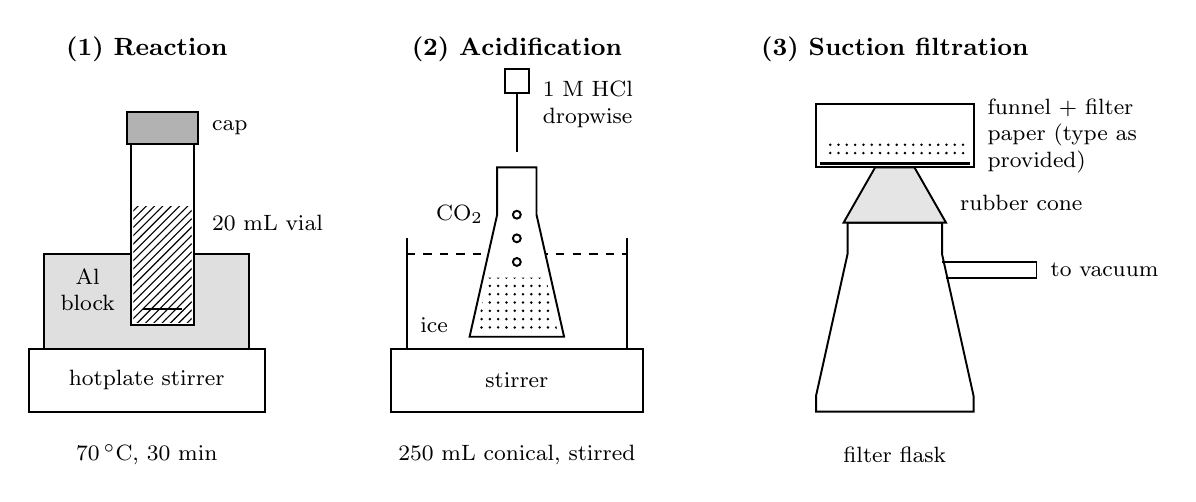
\begin{tikzpicture}[line width=0.7pt,font=\footnotesize]
% ---------- (1) vial in heating block
\begin{scope}[shift={(0,0)}]
 \node[font=\small\bfseries] at (1.5,4.6) {(1) Reaction};
 \draw (0,0) rectangle (3,0.8); \node at (1.5,0.4) {hotplate stirrer};
 \draw[fill=gray!25] (0.2,0.8) rectangle (2.8,2.0); \node[align=center] at (0.75,1.55) {Al\\block};
 \draw[fill=white] (1.3,1.1) rectangle (2.1,3.4);
 \draw[fill=gray!60] (1.25,3.4) rectangle (2.15,3.8);
 \node[right] at (2.2,3.6) {cap};
 \fill[pattern=north east lines] (1.33,1.13) rectangle (2.07,2.6);
 \draw (1.45,1.3) -- (1.95,1.3); \node[right] at (2.2,2.4) {20 mL vial};
 \node[align=left] at (1.5,-0.55) {70\,\si{\celsius}, 30 min};
\end{scope}
% ---------- (2) acidification
\begin{scope}[shift={(4.6,0)}]
 \node[font=\small\bfseries] at (1.6,4.6) {(2) Acidification};
 \draw (0,0) rectangle (3.2,0.8); \node at (1.6,0.4) {stirrer};
 \draw (0.2,0.8) -- (0.2,2.2) (3.0,0.8) -- (3.0,2.2);
 \draw[dashed] (0.2,2.0) -- (3.0,2.0); \node at (0.55,1.1) {ice};
 \draw[fill=white] (1.0,0.95) -- (2.2,0.95) -- (1.85,2.5) -- (1.85,3.1) -- (1.35,3.1) -- (1.35,2.5) -- cycle;
 \fill[pattern=dots] (1.08,1.0) -- (2.12,1.0) -- (1.97,1.7) -- (1.23,1.7) -- cycle;
 \draw (1.6,4.05) -- (1.6,3.3); \draw[fill=white] (1.45,4.05) rectangle (1.75,4.35);
 \node[right,align=left] at (1.8,3.9) {1 M HCl\\dropwise};
 \foreach \y in {1.9,2.2,2.5} \draw (1.6,\y) circle (0.05);
 \node[left] at (1.3,2.5) {\ce{CO2}};
 \node at (1.6,-0.55) {250 mL conical, stirred};
\end{scope}
% ---------- (3) suction filtration
\begin{scope}[shift={(9.4,0)}]
 \node[font=\small\bfseries] at (1.6,4.6) {(3) Suction filtration};
 \draw (0.6,0) -- (2.6,0) -- (2.6,0.2) -- (2.2,2.0) -- (2.2,2.4) -- (1.0,2.4) -- (1.0,2.0) -- (0.6,0.2) -- cycle;
 \draw (2.2,1.9) -- (3.4,1.9) -- (3.4,1.7) -- (2.25,1.7);
 \node[right] at (3.45,1.8) {to vacuum};
 \draw[fill=gray!20] (0.95,2.4) -- (2.25,2.4) -- (1.85,3.1) -- (1.35,3.1) -- cycle;
 \draw[fill=white] (0.6,3.1) rectangle (2.6,3.9);
 \draw[very thick] (0.65,3.15) -- (2.55,3.15);
 \fill[pattern=dots] (0.7,3.2) rectangle (2.5,3.45);
 \node[right,align=left] at (2.65,3.5) {funnel + filter\\paper (type as\\provided)};
 \node[right] at (2.3,2.65) {rubber cone};
 \node at (1.6,-0.55) {filter flask};
\end{scope}
\end{tikzpicture}
\end{center}

\vspace{4mm}
\begin{center}
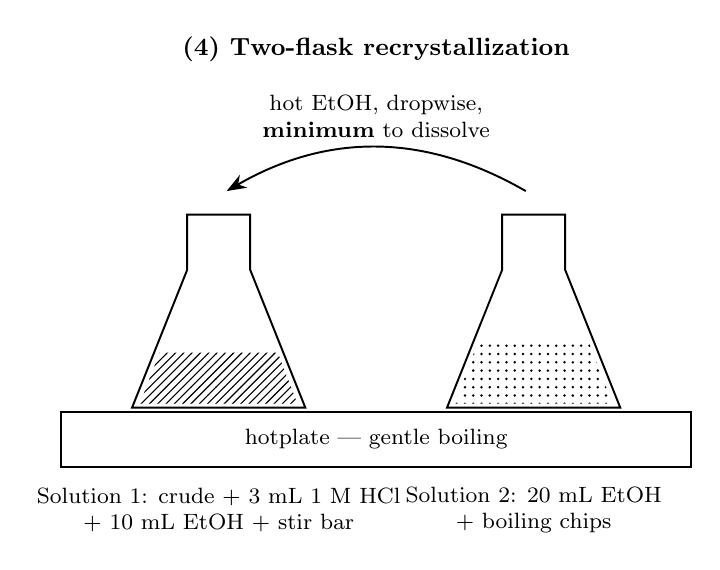
\begin{tikzpicture}[line width=0.7pt,font=\footnotesize]
\node[font=\small\bfseries] at (4,5.3) {(4) Two-flask recrystallization};
\draw (0,0) rectangle (8,0.7); \node at (4,0.35) {hotplate --- gentle boiling};
% flask 1
\draw[fill=white] (0.9,0.75) -- (3.1,0.75) -- (2.4,2.5) -- (2.4,3.2) -- (1.6,3.2) -- (1.6,2.5) -- cycle;
\fill[pattern=north east lines] (1.0,0.8) -- (3.0,0.8) -- (2.75,1.45) -- (1.25,1.45) -- cycle;
\node[align=center] at (2,-0.55) {Solution 1: crude + 3 mL 1 M HCl\\+ 10 mL EtOH + stir bar};
% flask 2
\draw[fill=white] (4.9,0.75) -- (7.1,0.75) -- (6.4,2.5) -- (6.4,3.2) -- (5.6,3.2) -- (5.6,2.5) -- cycle;
\fill[pattern=dots] (5.0,0.8) -- (7.0,0.8) -- (6.7,1.6) -- (5.3,1.6) -- cycle;
\node[align=center] at (6,-0.55) {Solution 2: 20 mL EtOH\\+ boiling chips};
% dropper
\draw[-{Stealth[length=2.5mm]}] (5.9,3.5) to[bend right=30] node[above,align=center]{hot EtOH, dropwise,\\\textbf{minimum} to dissolve} (2.1,3.5);
\end{tikzpicture}
\end{center}

\vspace{3mm}
\begin{callout}{ORDER OF EVENTS AFTER DISSOLUTION}
Clear solution \textrightarrow\ remove from heat \textrightarrow\ \textbf{undisturbed} to RT (10--15 min, larger and purer crystals) \textrightarrow\ ice 15 min (\textbf{solution 2 too}, as cold wash) \textrightarrow\ suction filter \textrightarrow\ wash with minimum cold EtOH \textrightarrow\ IR lamp 15 min.

\textbf{Tip (not in the manual).} If too much ethanol was added and few crystals form, gently boil off some ethanol on the hotplate and cool again; record this on the datasheet.
\end{callout}

\end{document}
